\section{\tl{OPNMF vs OPNMF - DCCA}}
\en{
Furthermore, we explore the effect that OPNMF has to the task of classification. To that extent, we compare the classification results of (a) the data after the imaging view has been transformed with OPNMF and (b) the DCCA transformed data, trained on the raw genetic data and the OPNMF transformed imaging data.

}
\subsection{\en{Without scaling or balancing:}}
\en{
\begin{figure}[H]
    \centering
    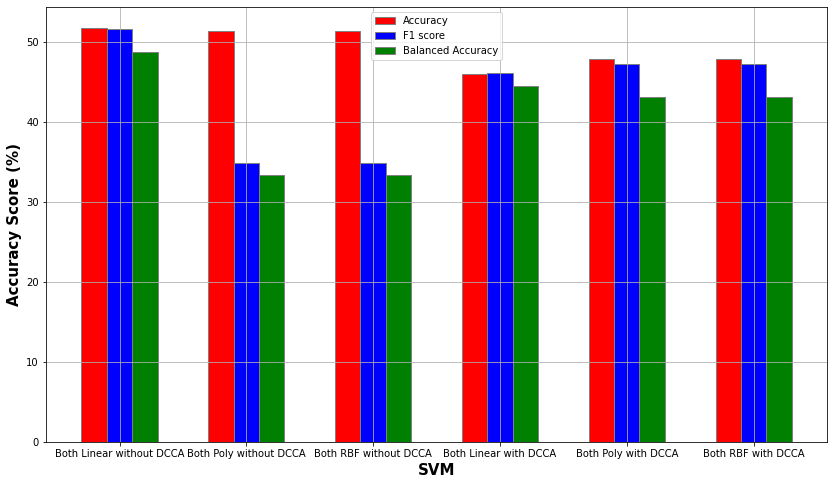
\includegraphics[width=\textwidth]{figures/Results/NMF/NMF_Both_out.png}
    \caption[\en{Classification metric scores using Both views on OPNMF vs OPNMF-DCCA data}]{\en{Classification metric scores using Both views (Imaging and Genetic), on the SVM kernels (Linear, Polynomial, RBF), using raw genetic and OPNMF transformed imaging data (3 left bar groups) vs using DCCA transformed raw genetic and OPNMF transformed imaging data (3 right bar groups)}}
\end{figure}

\begin{figure}[H]
    \centering
    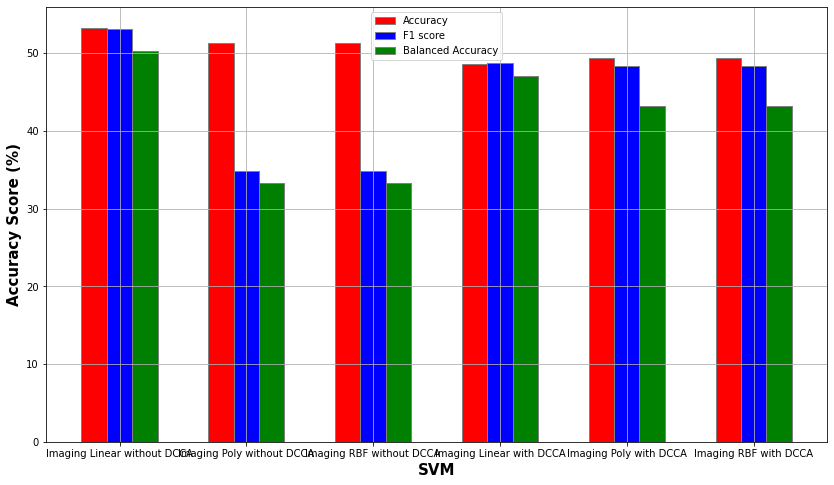
\includegraphics[width=\textwidth]{figures/Results/NMF/NMF_Ima_out.png}
    \caption[\en{Classification metric scores using Imaging view on OPNMF vs OPNMF-DCCA data}]{\en{Classification metric scores using only the Imaging view, on the SVM kernels (Linear, Polynomial, RBF), using OPNMF transformed imaging data (3 left bar groups) vs using the DCCA transformed imaging data, trained on raw genetic data and OPNMF transformed genetic data (3 right bar groups).}}
\end{figure}

\begin{figure}[H]
    \centering
    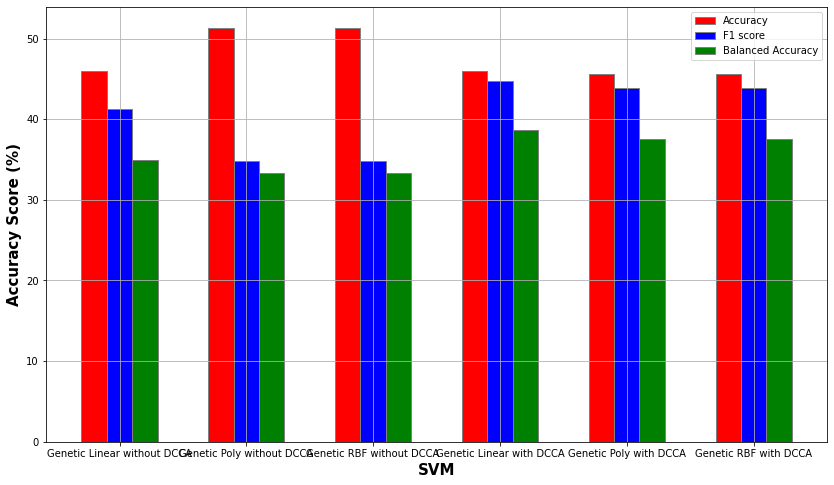
\includegraphics[width=\textwidth]{figures/Results/NMF/NMF_Gen_out.png}
    \caption[\en{Classification metric scores using Genetic view on OPNMF vs OPNMF-DCCA data}]{\en{Classification metric scores using only the Imaging view, on the SVM kernels (Linear, Polynomial, RBF), using OPNMF transformed imaging data (3 left bar groups) vs using the DCCA transformed imaging data, trained on raw genetic data and OPNMF transformed genetic data (3 right bar groups).}}
\end{figure}

% \begin{figure}[H]
%     \centering
%     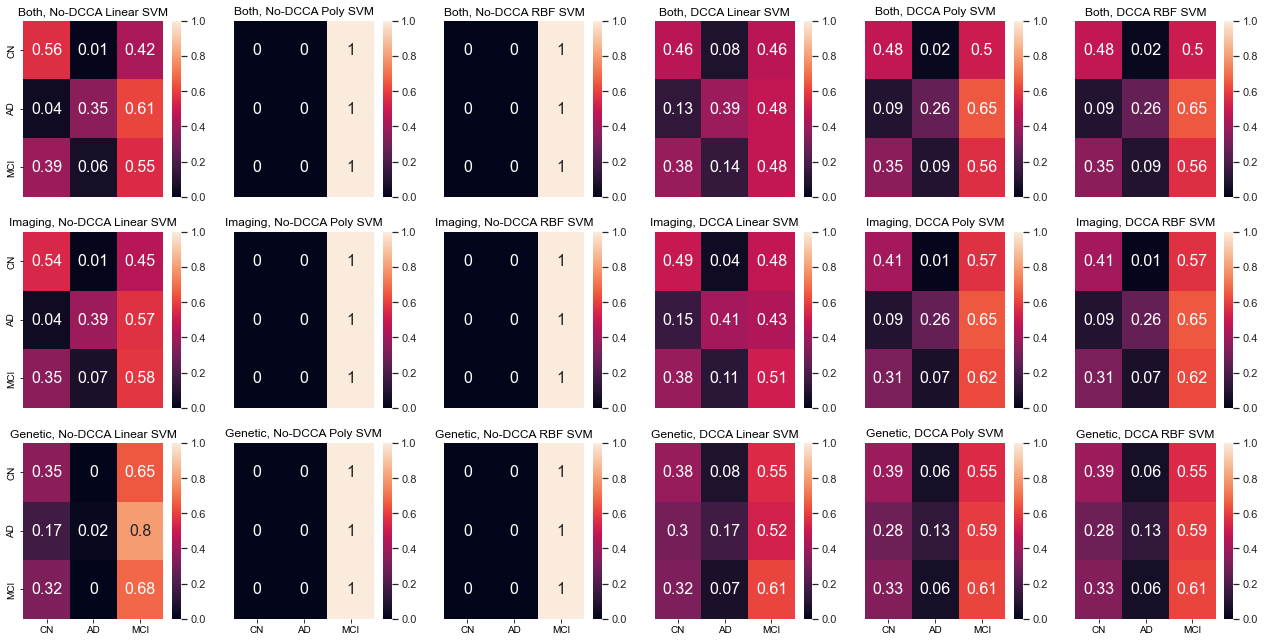
\includegraphics[width=\textwidth]{figures/Results/NMF/NMF_CM_out.png}
%     \caption[\en{Confusion Matrices of OPNMF vs OPNMF-DCCA data}]{\en{Classification metric scores using only the Imaging view, on the SVM kernels (Linear, Polynomial, RBF), using OPNMF transformed imaging data (3 left bar groups) vs using the DCCA transformed imaging data, trained on raw genetic data and OPNMF transformed genetic data (3 right bar groups).}}
% \end{figure}

\begin{figure}[H]
    \centering
    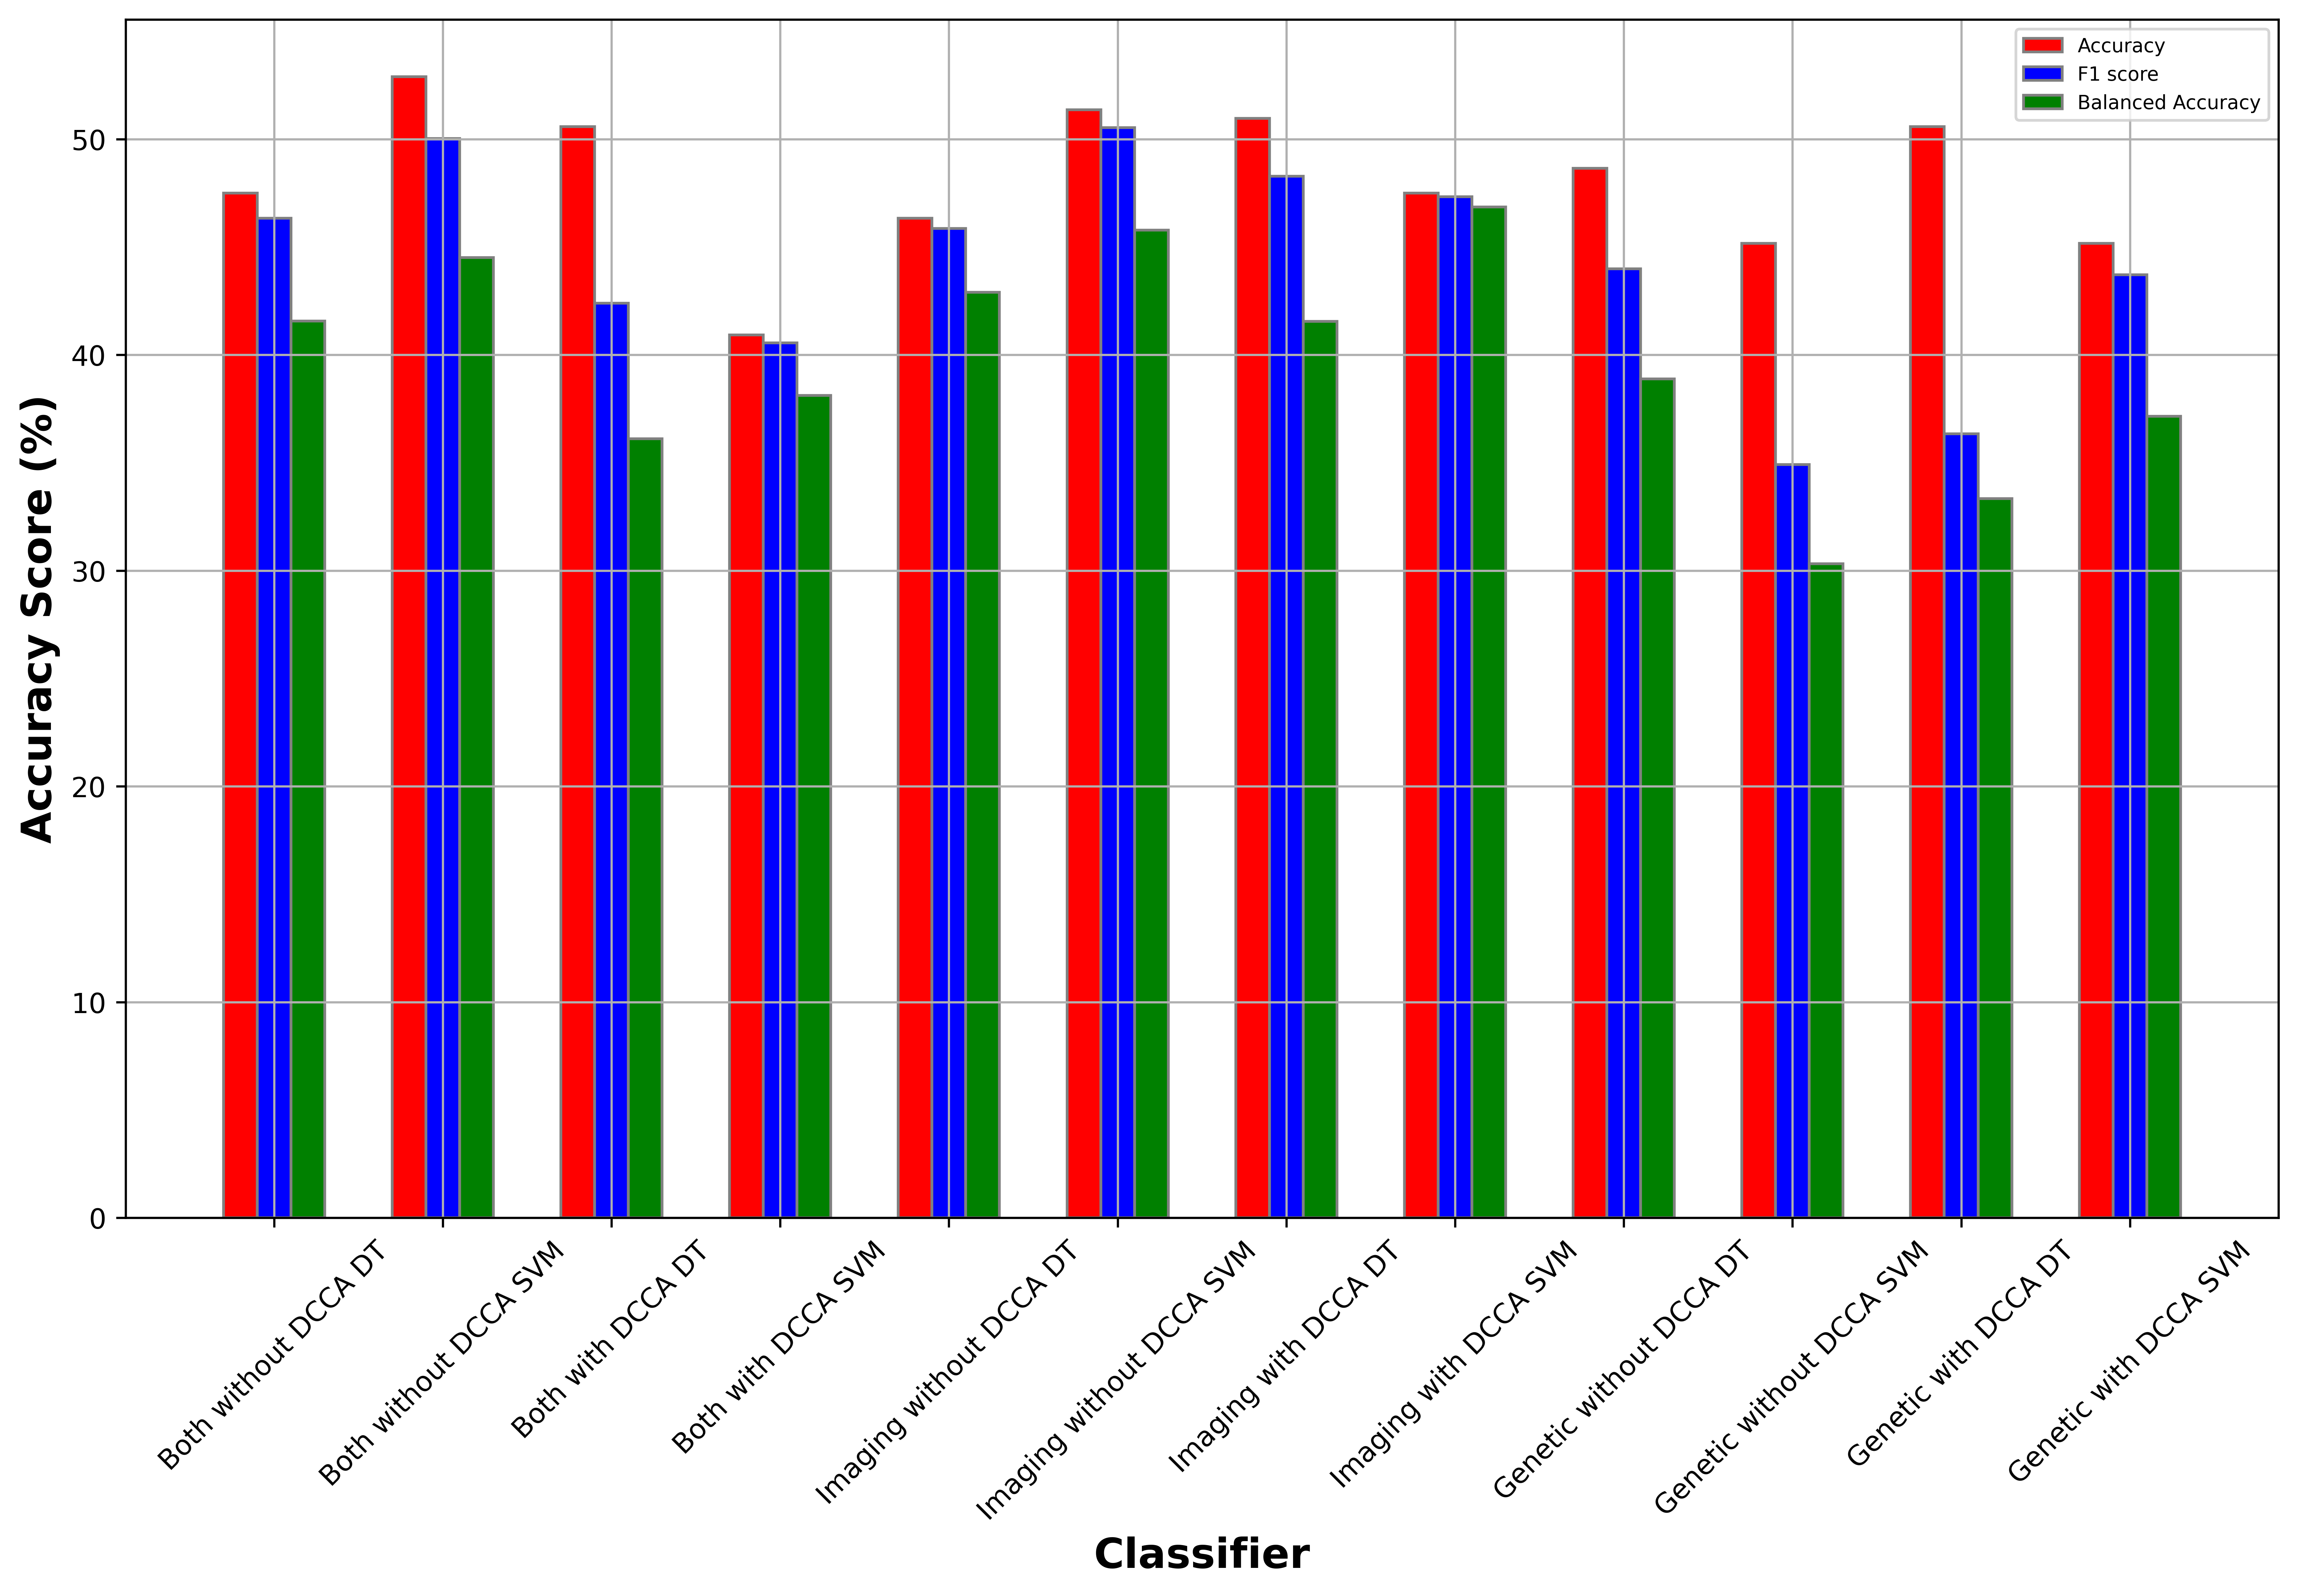
\includegraphics[width=\textwidth]{figures/Results/NMF/Bagging_NMF_out.png}
    \caption[\en{OPNMF Bagging Classification metrics}]{\en{Classification metric using Bagging on the OPNMF transformed imaging and genetic data.}}
\end{figure}

% \begin{figure}[H]
%     \centering
%     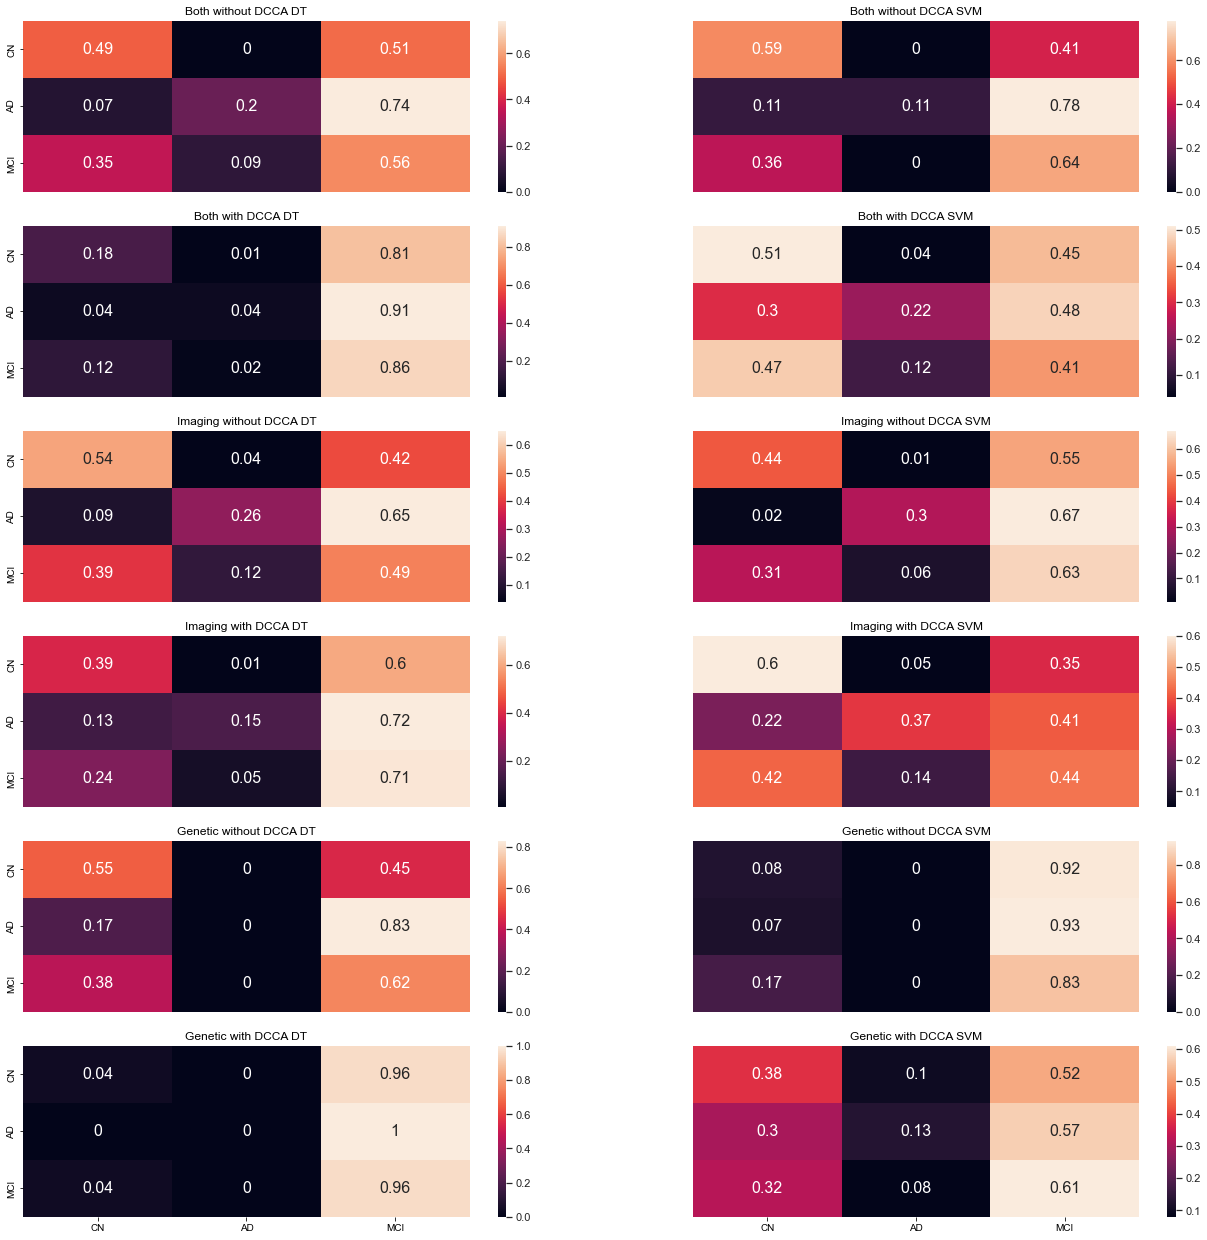
\includegraphics[width=\textwidth]{figures/Results/NMF/Bagging_NMF_CM_out.png}
%     \caption[\en{OPNMF Bagging Confusion Matrices}]{\en{The Confusion Matrices for each class, with Bagging, for the OPNMF transformed imaging and genetic data.}}
% \end{figure}

\begin{figure}[H]
    \centering
    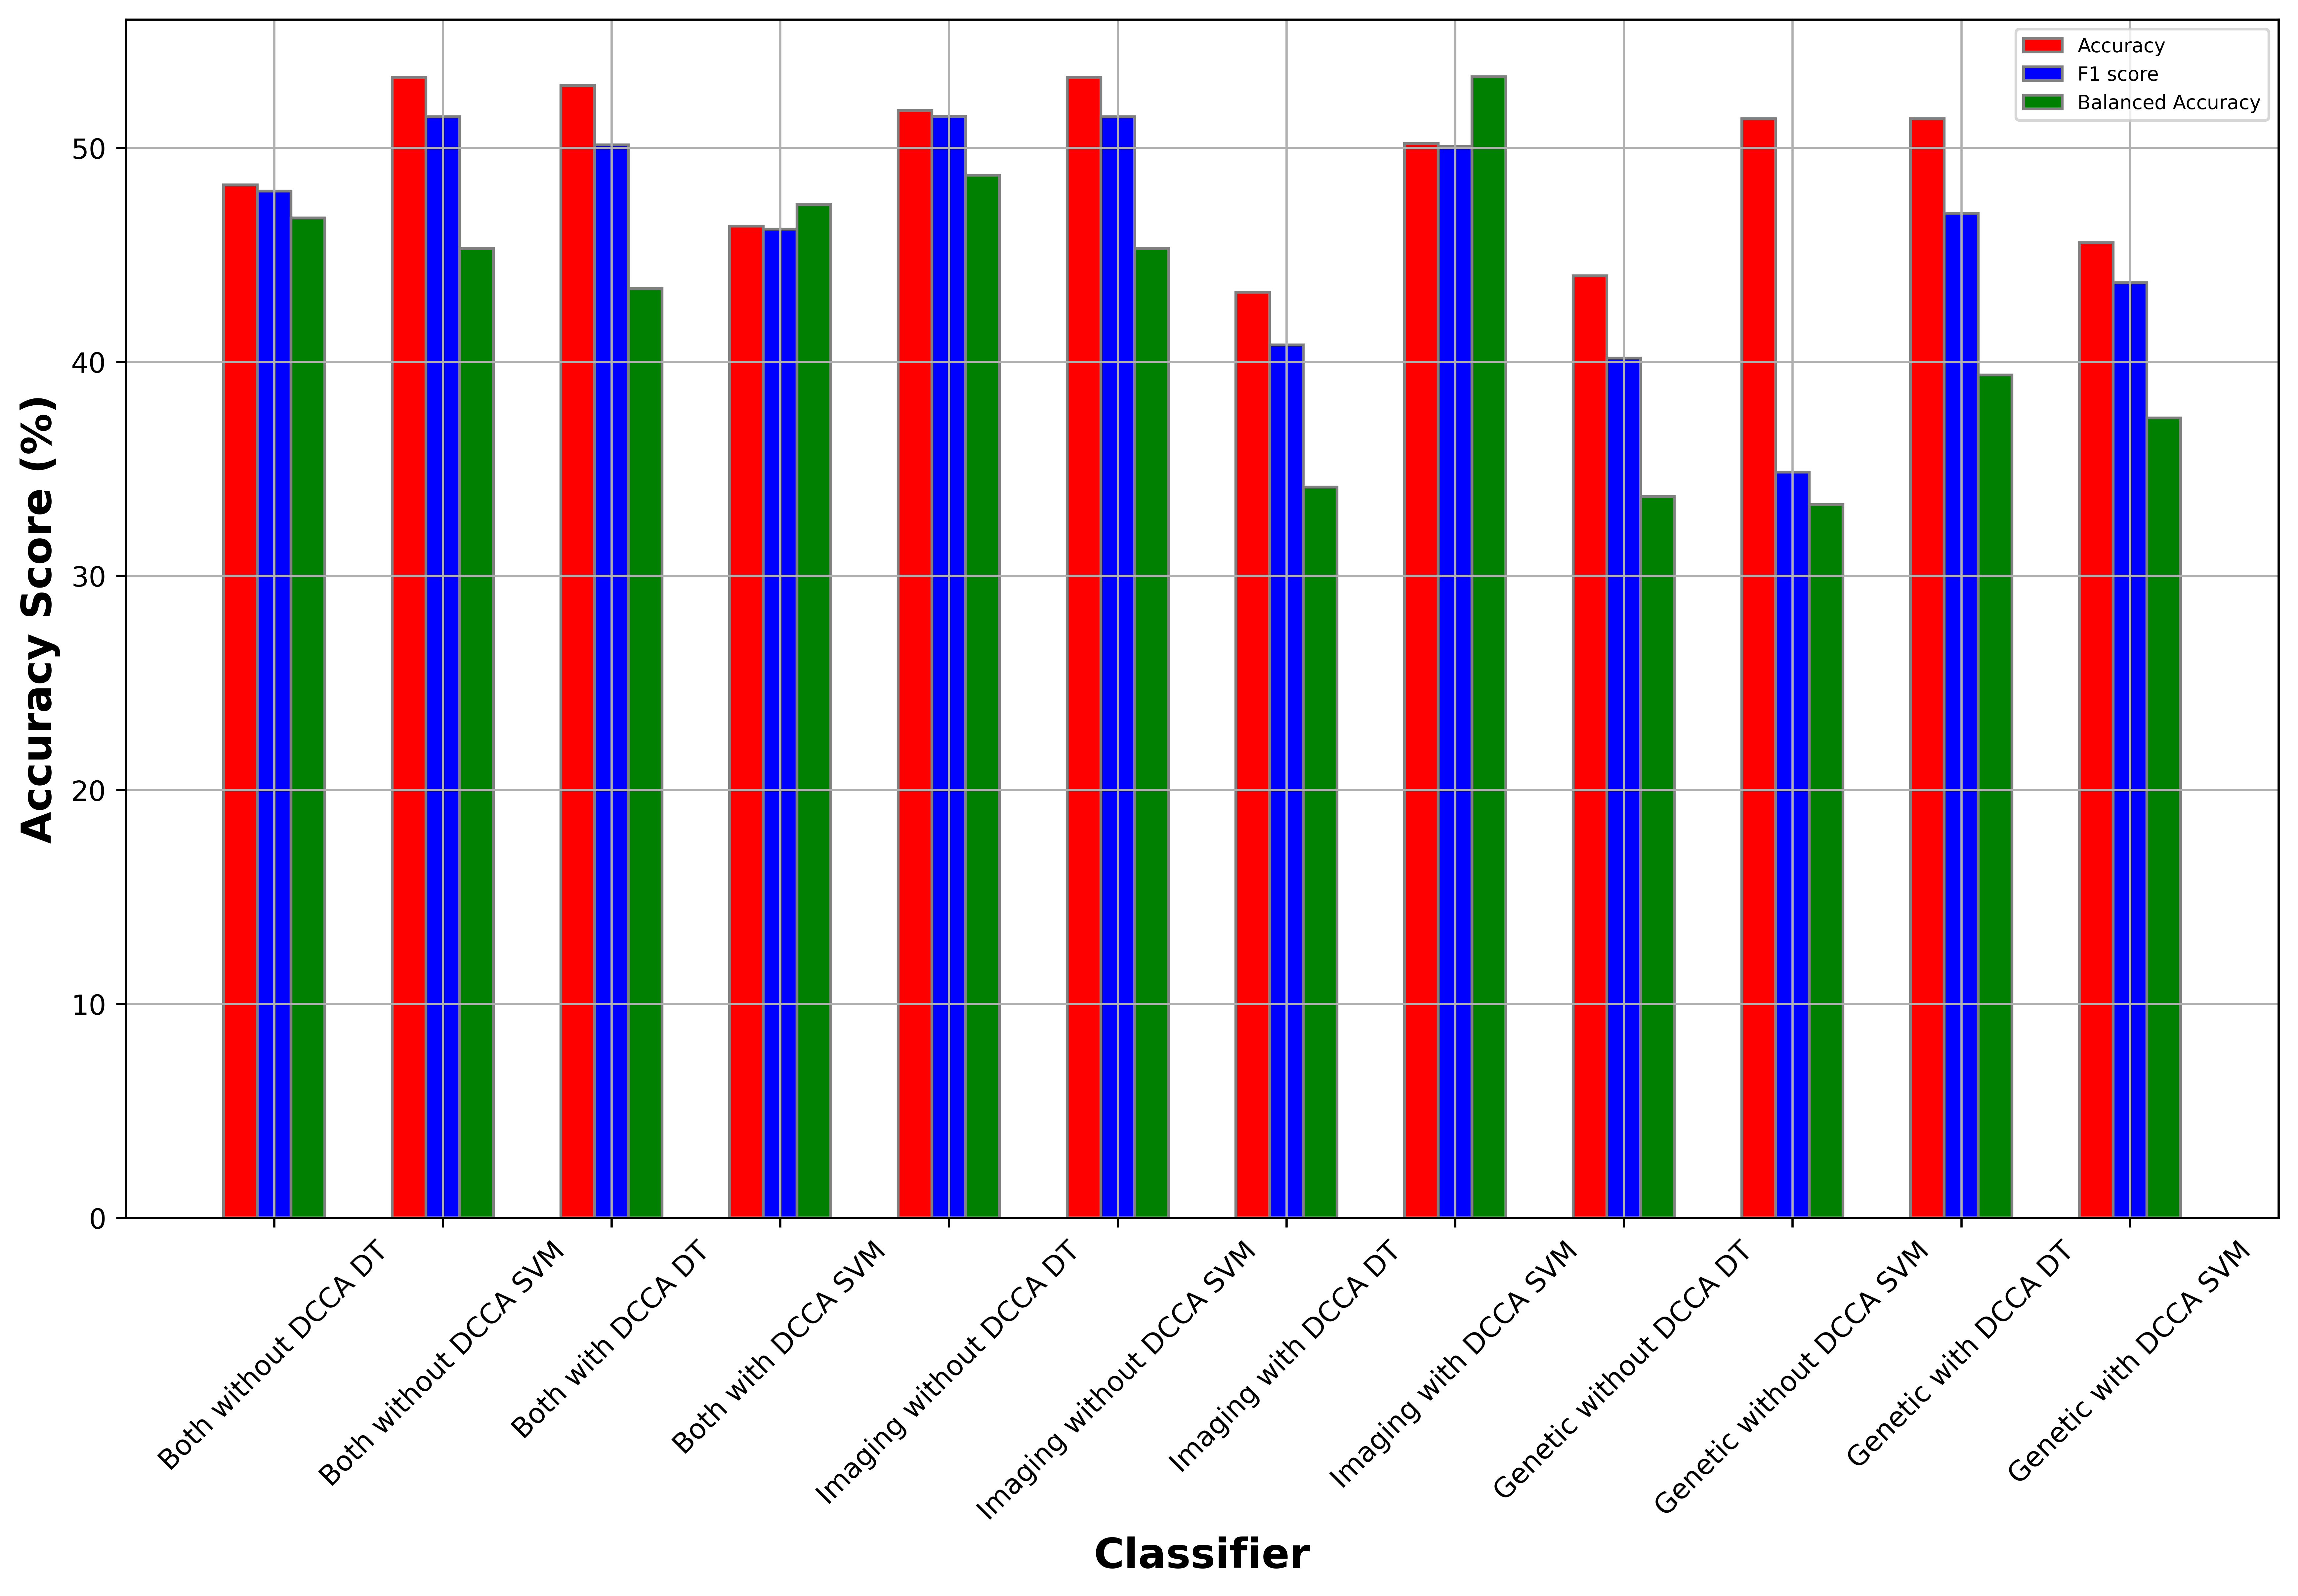
\includegraphics[width=\textwidth]{figures/Results/NMF/AdaBoost_NMF_out.png}
    \caption[\en{OPNMF AdaBoost Classification metrics}]{\en{Classification metric using AdaBoost on the OPNMF transformed imaging and genetic data.}}
\end{figure}

% \begin{figure}[H]
%     \centering
%     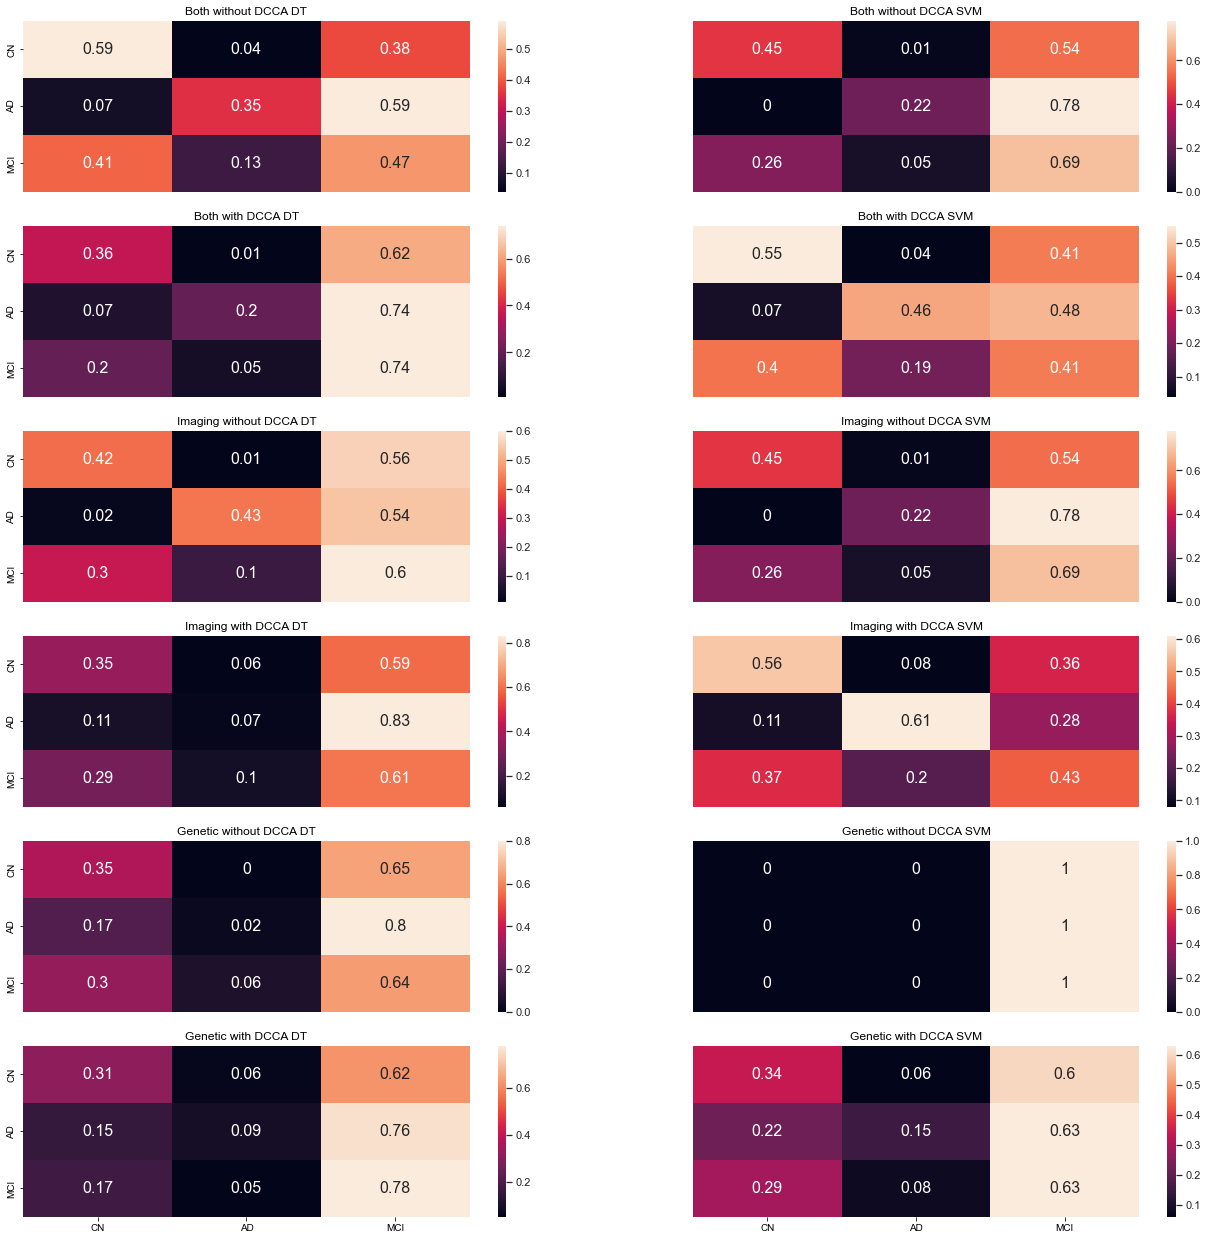
\includegraphics[width=\textwidth]{figures/Results/NMF/AdaBoost_NMF_CM_out.png}
%     \caption[\en{OPNMF AdaBoost Confusion Matrices}]{\en{The Confusion Matrices for each class, with AdaBoost, for the OPNMF transformed imaging and genetic data.}}
% \end{figure}
}
\subsection{\en{With scaling and balancing:}}
\en{
\begin{figure}[H]
    \centering
    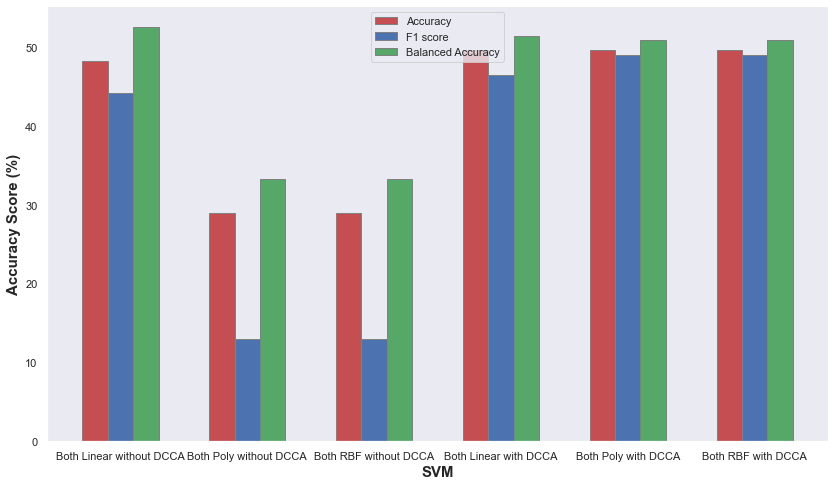
\includegraphics[width=\textwidth]{figures/Results/NMF/NMF_Both_with.png}
    \caption[\en{Classification metric scores using Both views on OPNMF vs OPNMF-DCCA data }]{\en{Classification metric scores using Both views (Imaging and Genetic), on the SVM kernels (Linear, Polynomial, RBF), using raw genetic and OPNMF transformed imaging data (3 left bar groups) vs using DCCA transformed raw genetic and OPNMF transformed imaging data (3 right bar groups)}}
\end{figure}

\begin{figure}[H]
    \centering
    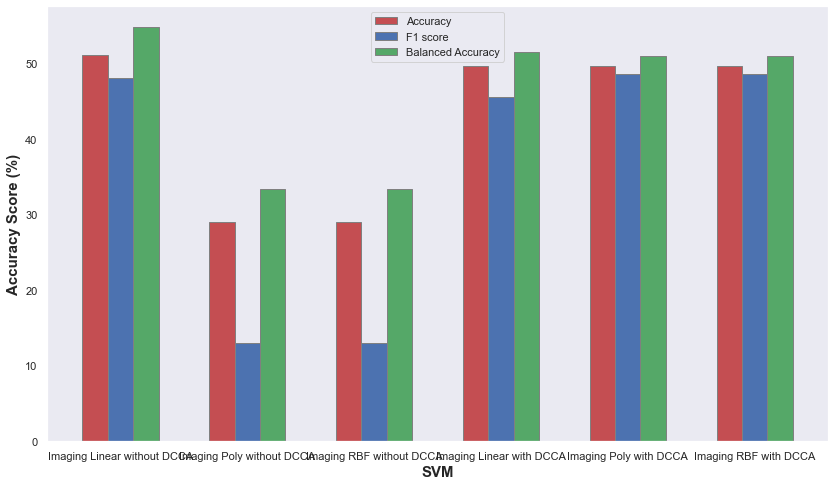
\includegraphics[width=\textwidth]{figures/Results/NMF/NMF_Ima_with.png}
    \caption[\en{Classification metric scores using Imaging view on OPNMF vs OPNMF-DCCA data }]{\en{Classification metric scores using only the Imaging view, on the SVM kernels (Linear, Polynomial, RBF), using OPNMF transformed imaging data (3 left bar groups) vs using the DCCA transformed imaging data, trained on raw genetic data and OPNMF transformed genetic data (3 right bar groups).}}
\end{figure}

\begin{figure}[H]
    \centering
    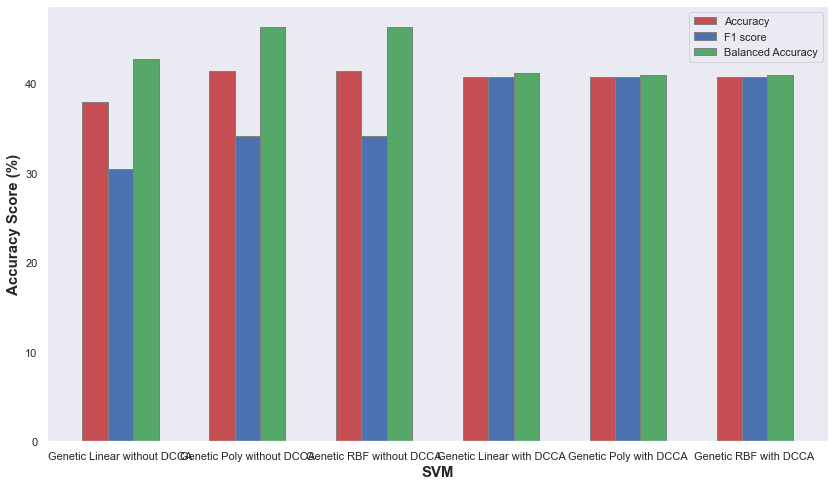
\includegraphics[width=\textwidth]{figures/Results/NMF/NMF_Gen_with.png}
    \caption[\en{Classification metric scores using Genetic view on OPNMF vs OPNMF-DCCA data }]{\en{Classification metric scores using only the genetic view, on the SVM kernels (Linear, Polynomial, RBF), using raw genetic data (3 left bar groups) vs using the DCCA transformed genetic data, trained on raw genetic data and OPNMF transformed imaging data (3 right bar groups).}}
\end{figure}

% \begin{figure}[H]
%     \centering
%     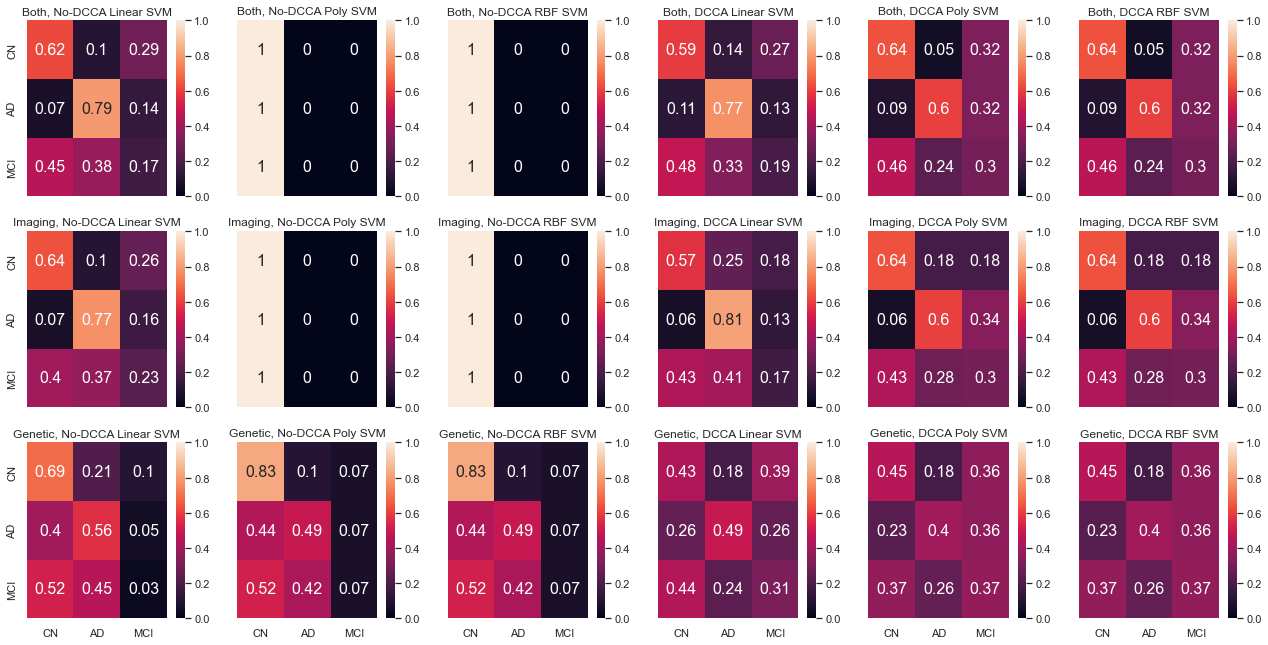
\includegraphics[width=\textwidth]{figures/Results/NMF/NMF_CM_with.png}
%     \caption[\en{Confusion Matrices of OPNMF vs OPNMF-DCCA data with scaling and balancing}]{\en{The Confusion Matrices for each class, per model, using both views (top row), only the imaging view (middle row), and only the genetic view (bottom row). The three left columns represent the CM of the raw genetic and OPNMF transformed imaging data classification, while the three right columns represent the CM of the DCCA transformed data classification.}}
% \end{figure}

\begin{figure}[H]
    \centering
    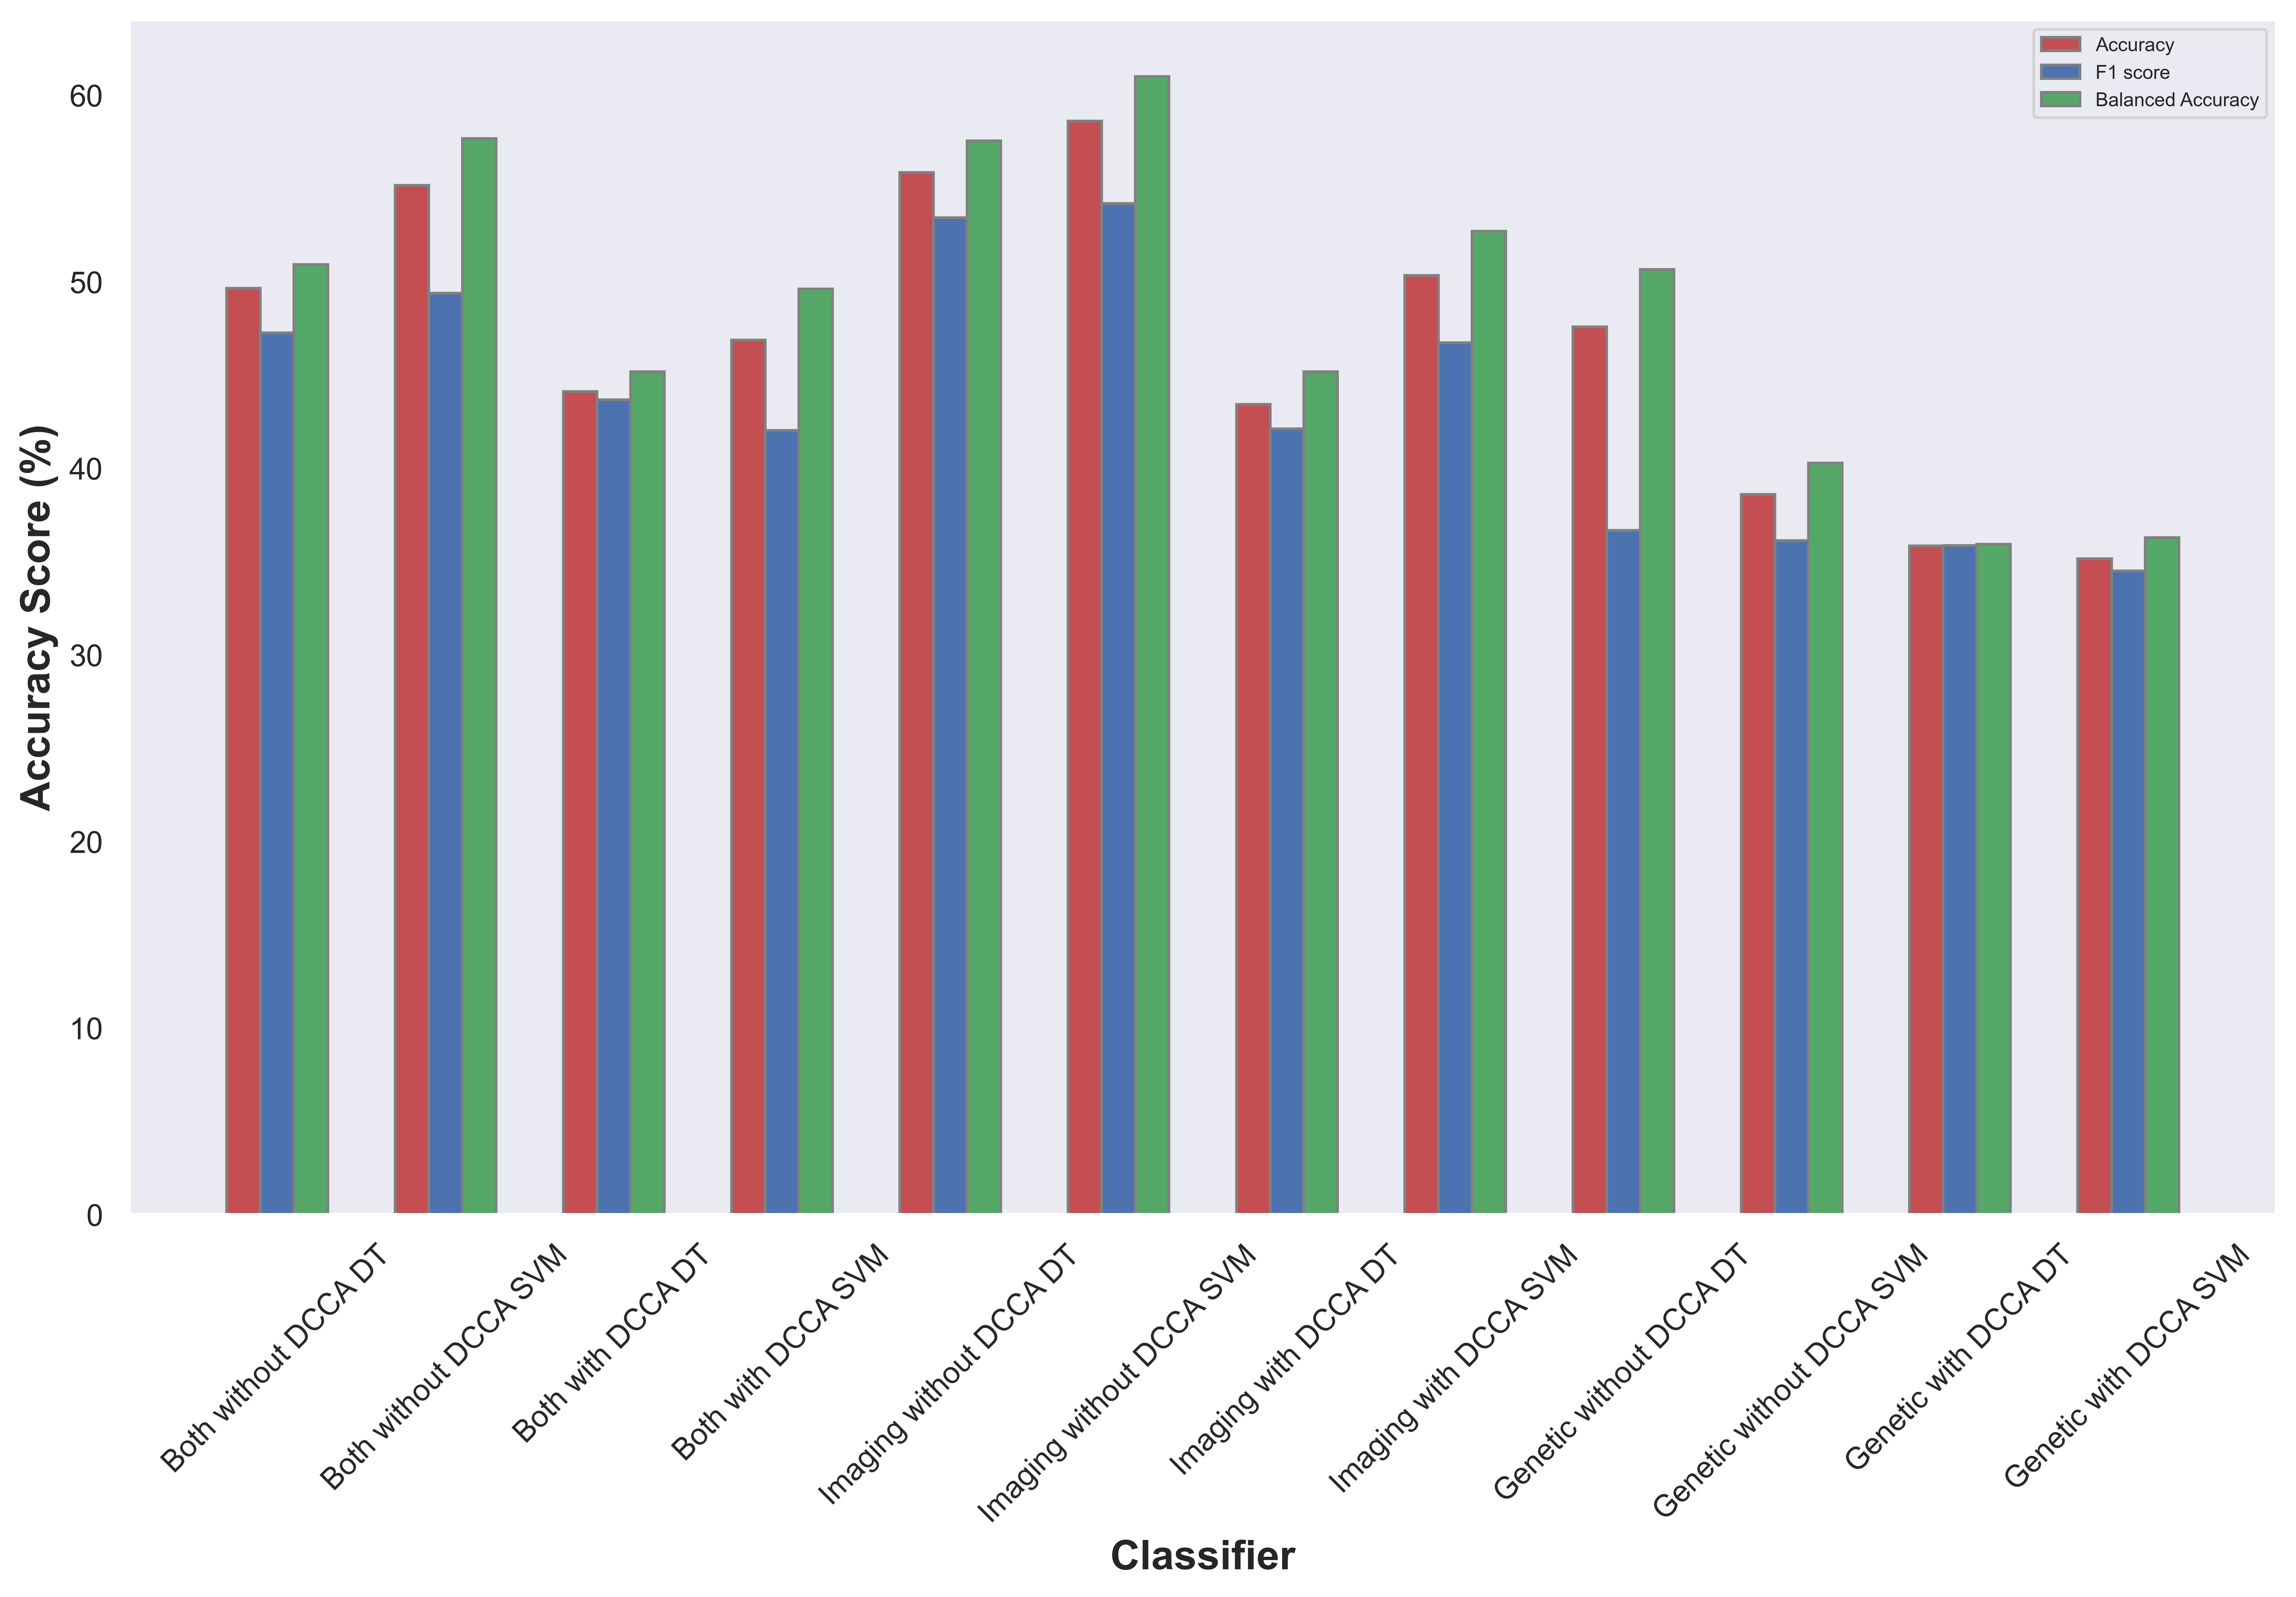
\includegraphics[width=\textwidth]{figures/Results/NMF/Bagging_NMF_with.png}
    \caption[\en{OPNMF Bagging Classification metrics with scaling and balancing}]{\en{Classification metric using Bagging on the OPNMF transformed imaging and genetic data.}}
\end{figure}

\begin{figure}[H]
    \centering
    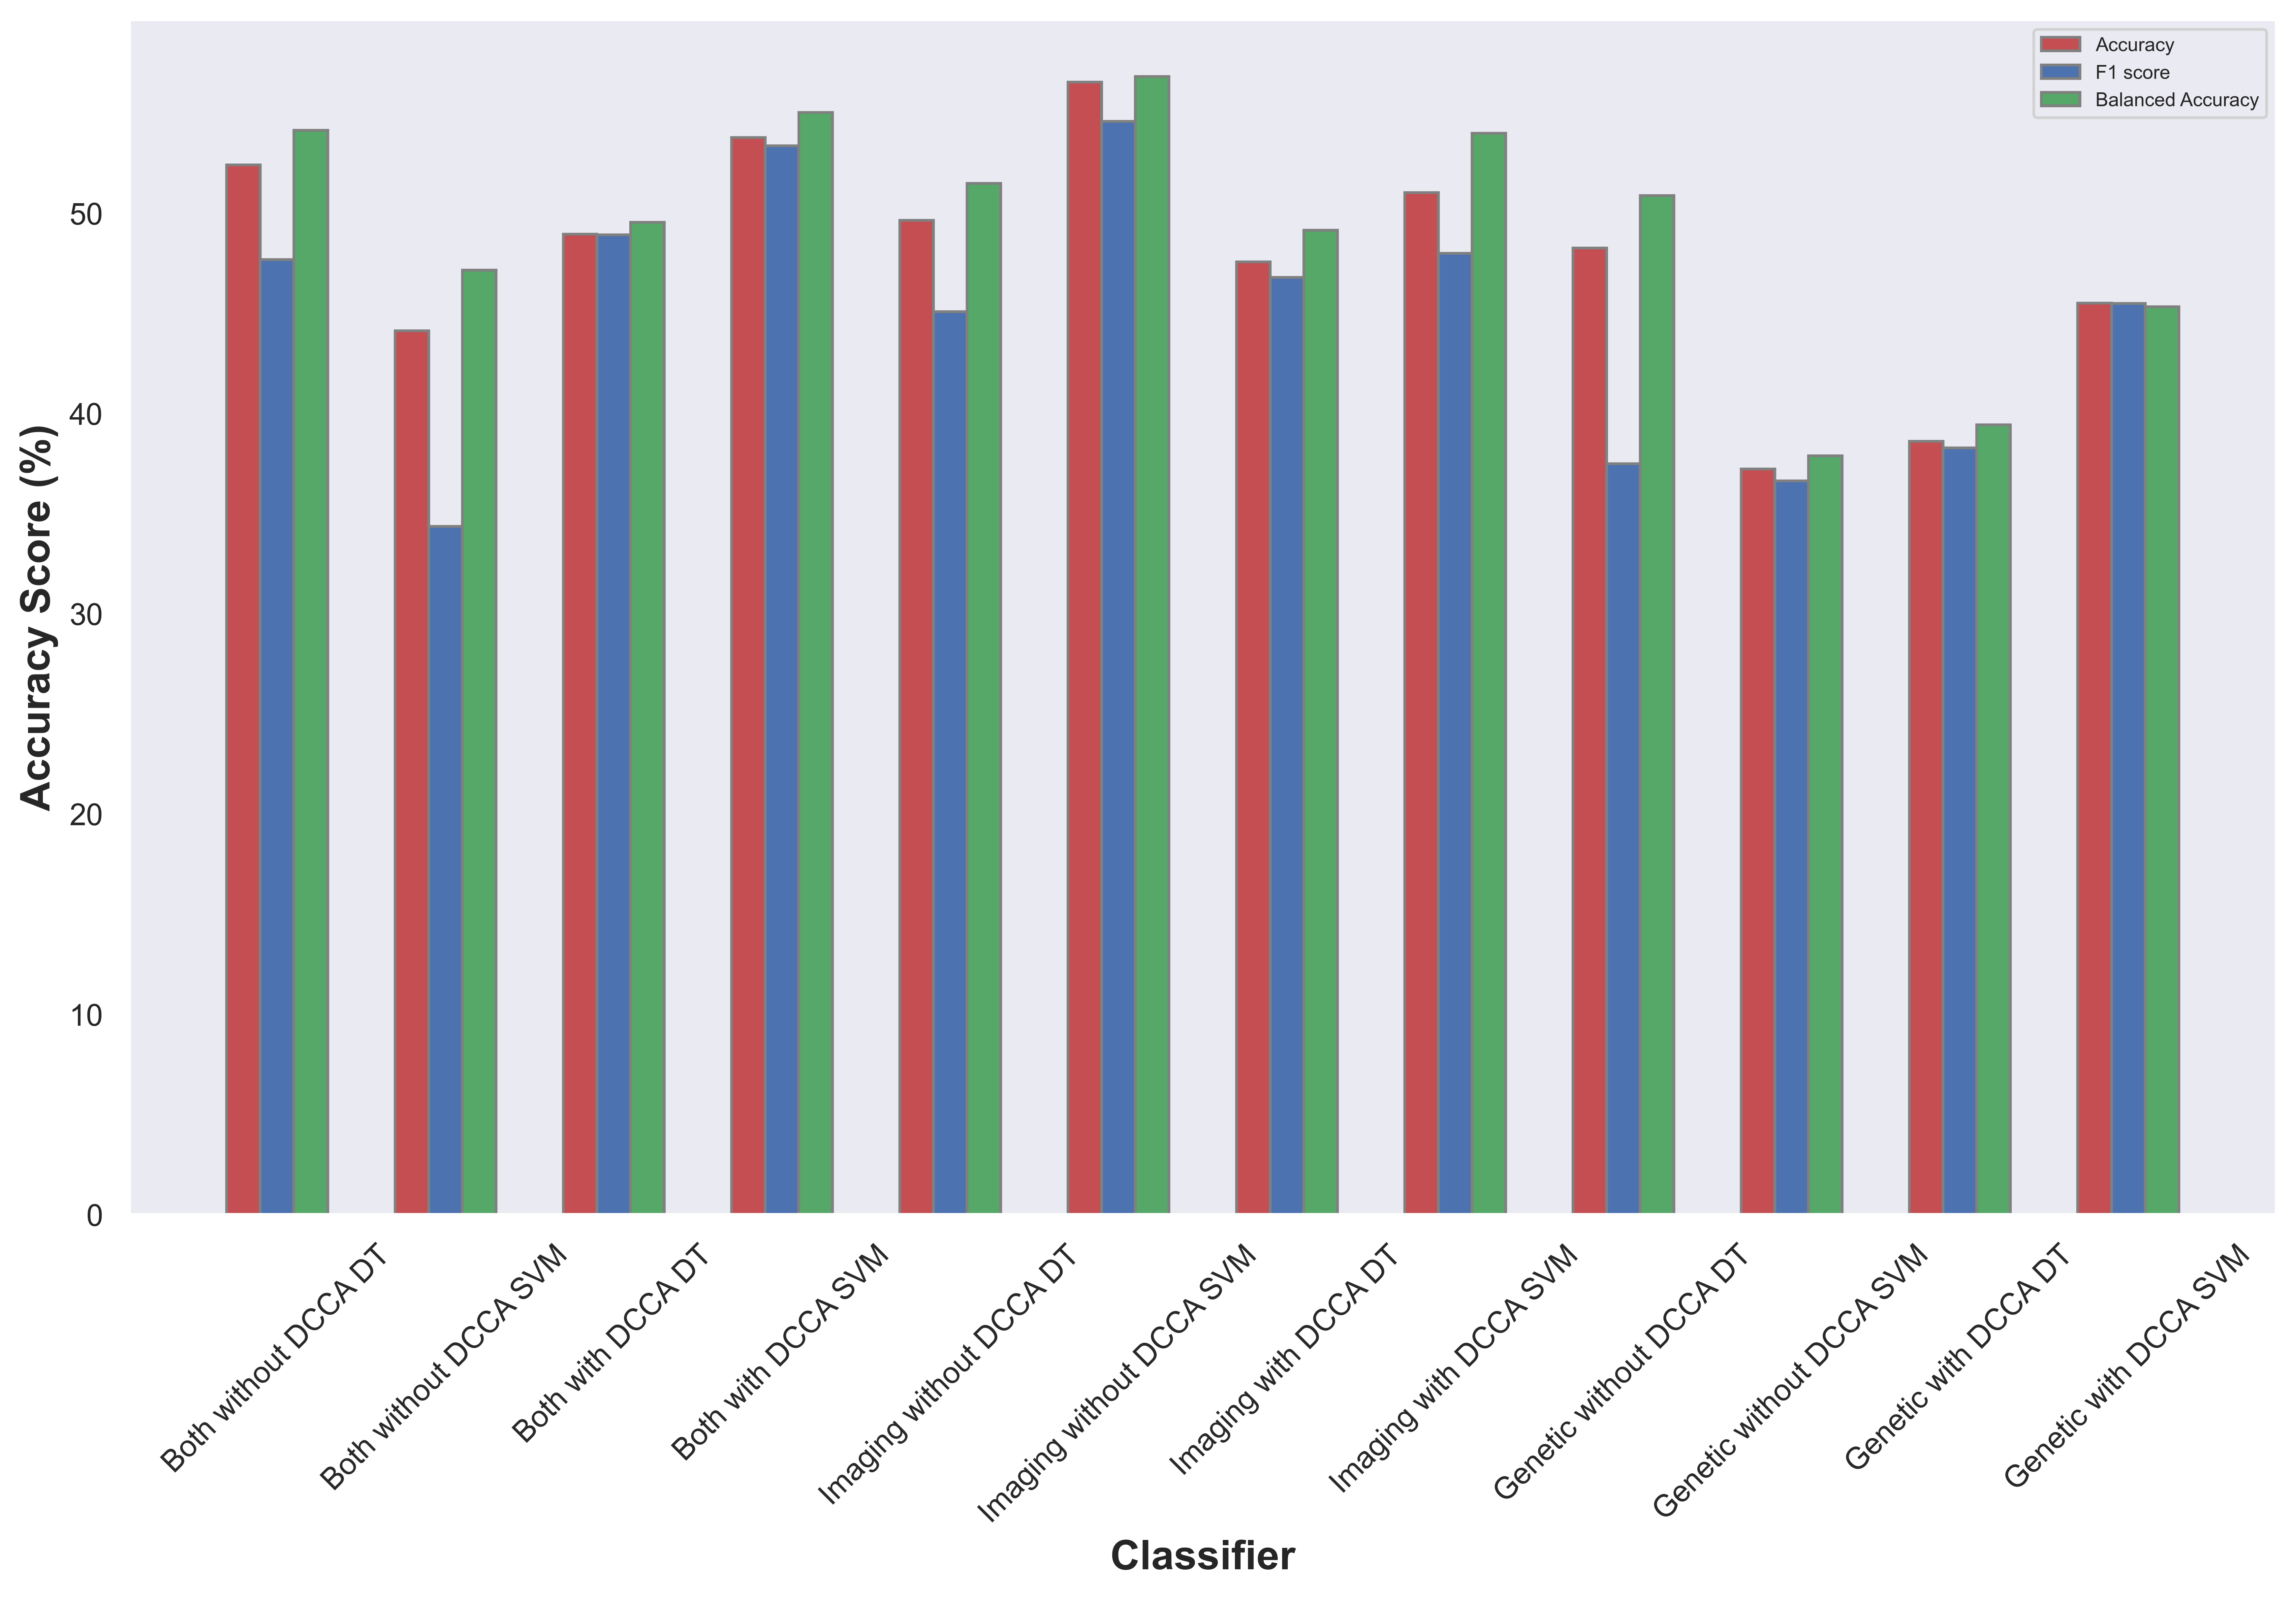
\includegraphics[width=\textwidth]{figures/Results/NMF/AdaBoost_NMF_with.png}
    \caption[\en{OPNMF AdaBoost Classification metrics with scaling and balancing}]{\en{Classification metric using AdaBoost on the OPNMF transformed imaging and genetic data.}}
\end{figure}

The confusion matrices of the OPNMF Bagging models are shown, because they performed exceptionally good:
\begin{figure}[H]
    \centering
    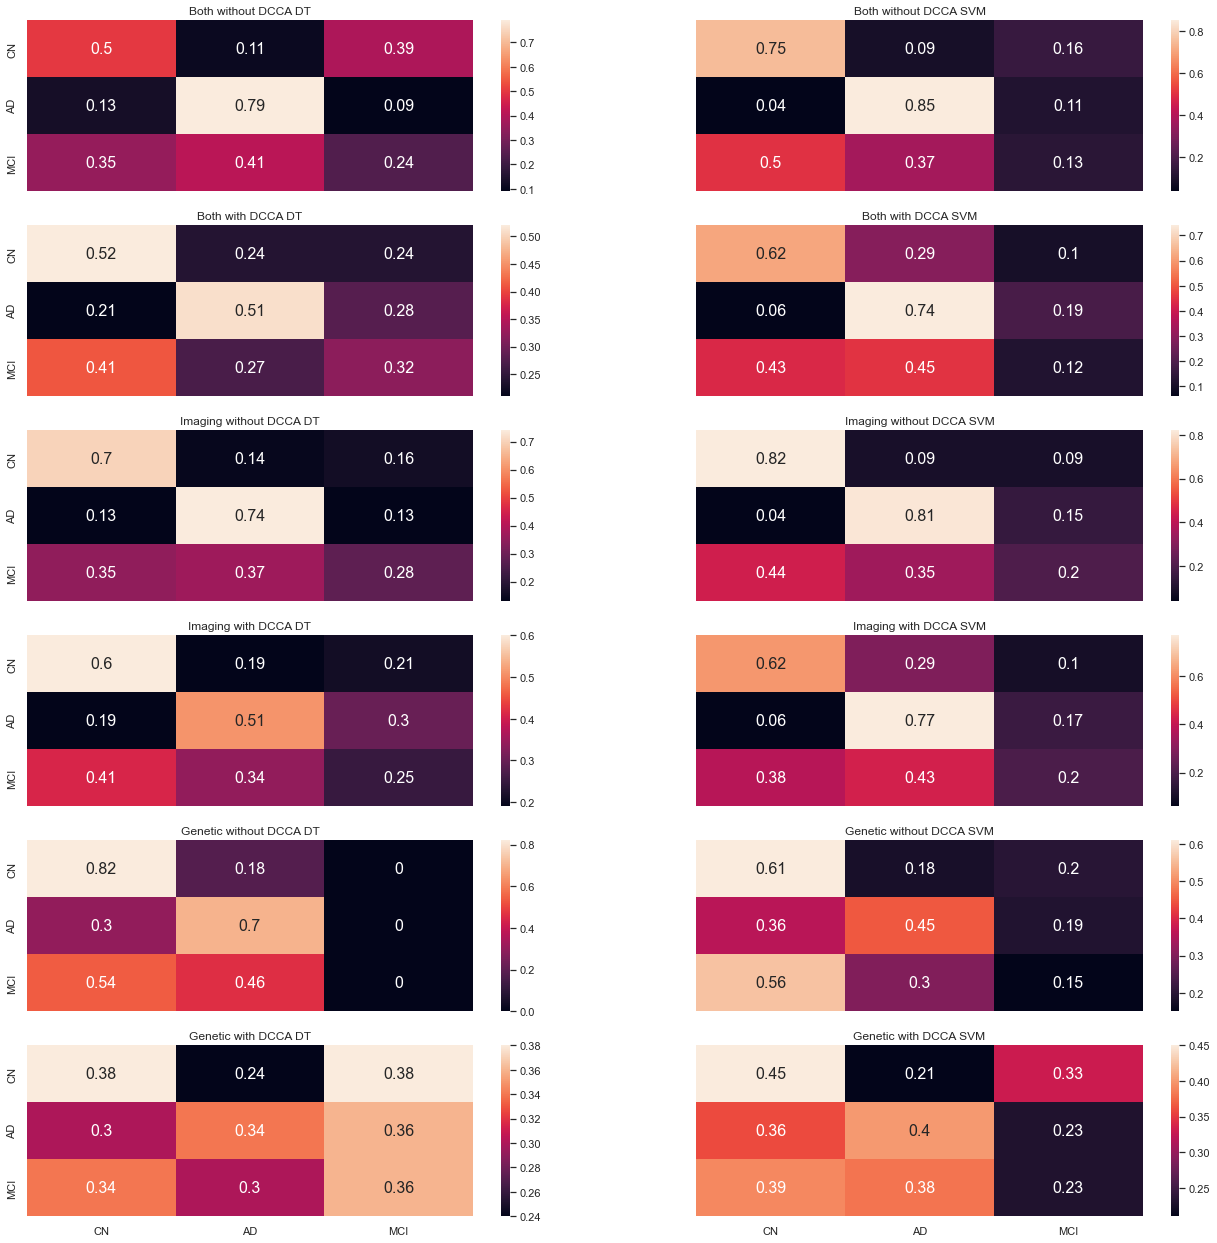
\includegraphics[width=\textwidth]{figures/Results/NMF/Bagging_NMF_CM_with.png}
    \caption[\en{OPNMF Bagging Confusion Matrices with scaling and balancing}]{\en{The Confusion Matrices for each class, with Bagging, for the OPNMF transformed imaging and genetic data.}}
    \label{fig:OPNMF Bagging Confusion Matrices with scaling and balancing}
\end{figure}

\begin{figure}[H]
    \centering
    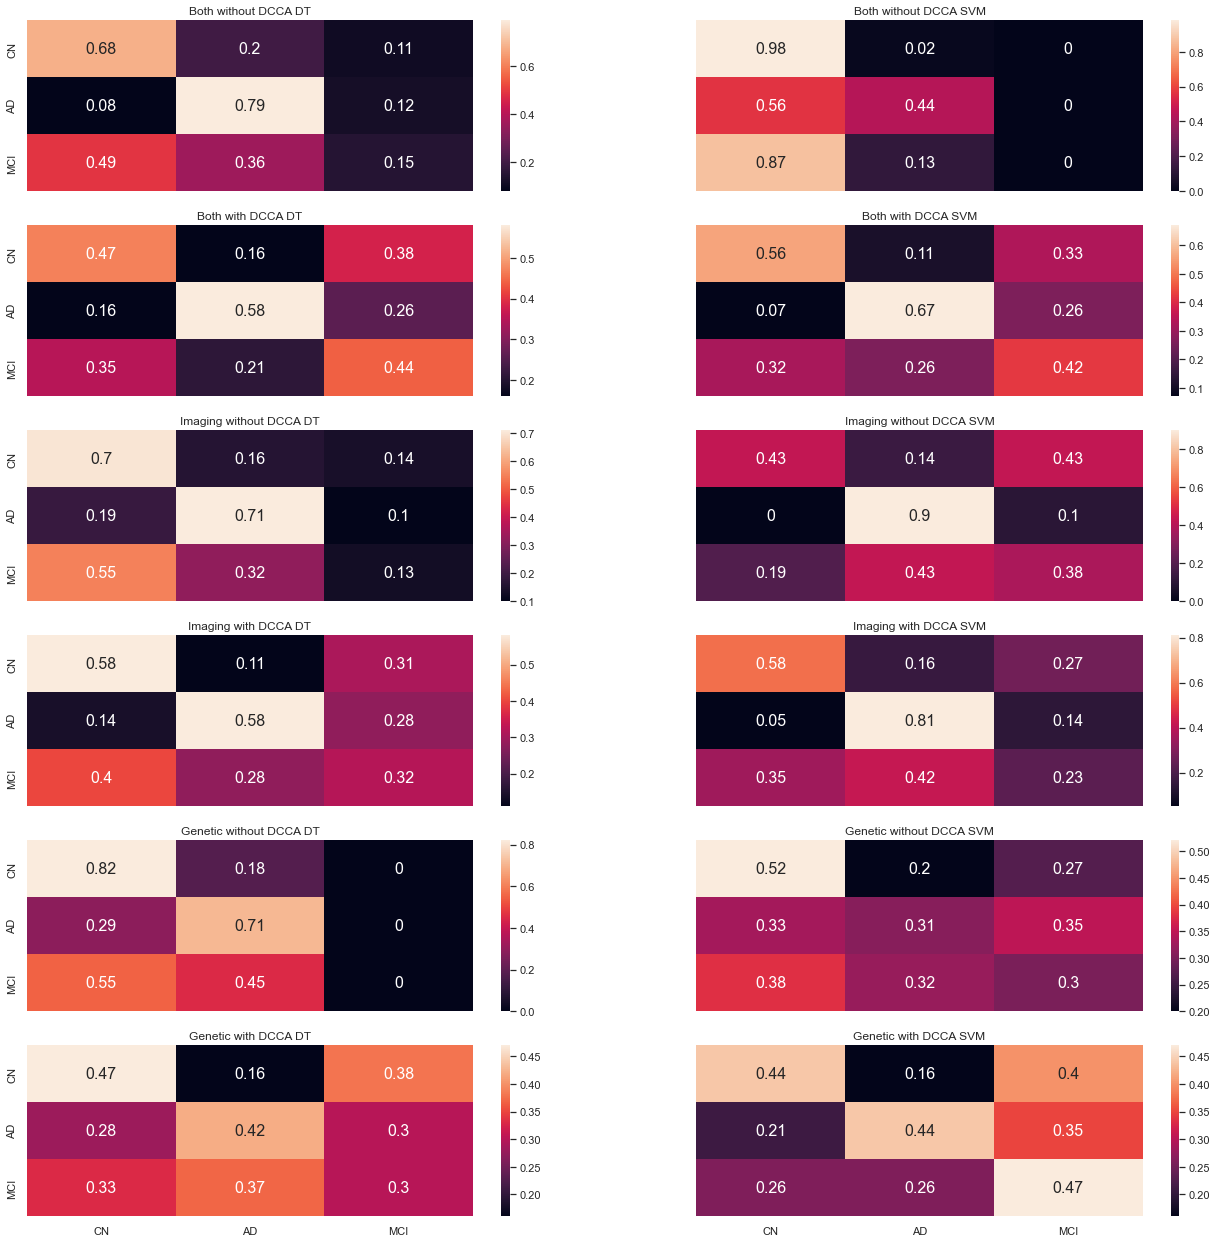
\includegraphics[width=\textwidth]{figures/Results/NMF/AdaBoost_NMF_CM_with.png}
    \caption[\en{OPNMF AdaBoost Confusion Matrices with scaling and balancing}]{\en{The Confusion Matrices for each class, with AdaBoost, for the OPNMF transformed imaging and genetic data.}}
    \label{fig:OPNMF AdaBoost Confusion Matrices with scaling and balancing}
\end{figure}

The following tables present the complete results for the OPNMF transformed data, as well as the DCCA transformed data after OPMNF transformation on the imaging data, for each model, for each metric, for each view, and either with or without scaling and balancing. With green are highlighted the best values for each metric, depending on whether scaling and balancing were applied:

\begin{figure} [H]
    \centering
    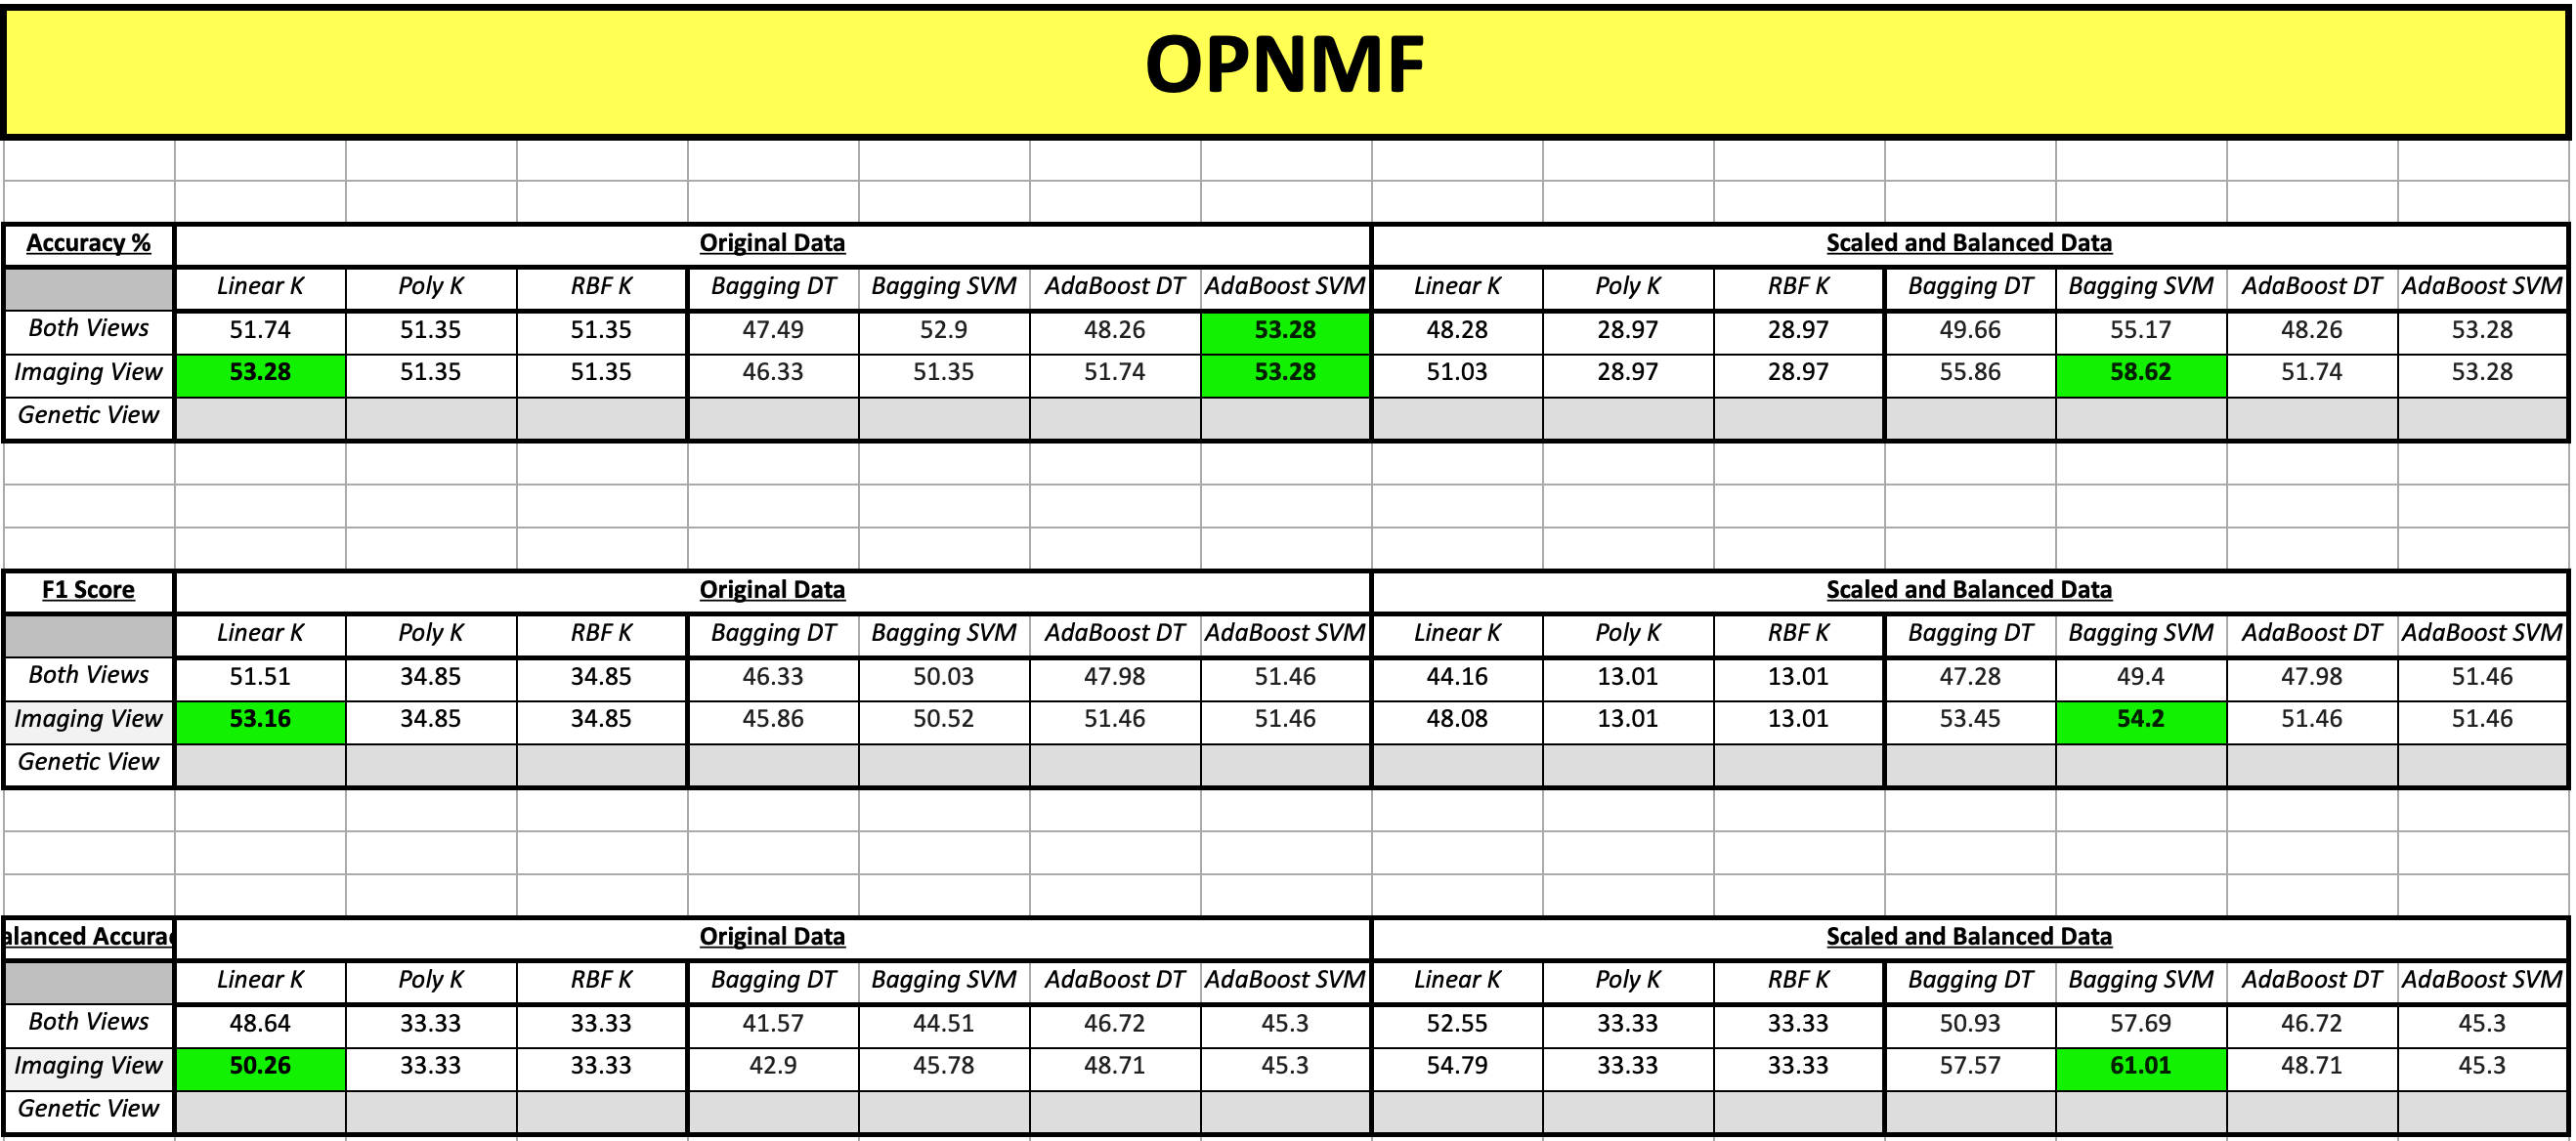
\includegraphics[width=\textwidth]{figures/Results/Analytical_Table_OPNMF.png}
    \caption[\en{Analytical table of results for OPNMF data classification}]{\en{For each model and classifier, the metric scores for OPNMF transformed data classification are presented. Highlighted green are the best performing models, for each metric.}}
    \label{fig: Summary Table for classification scores for OPNMF transformed data}
\end{figure}

\begin{figure} [H]
    \centering
    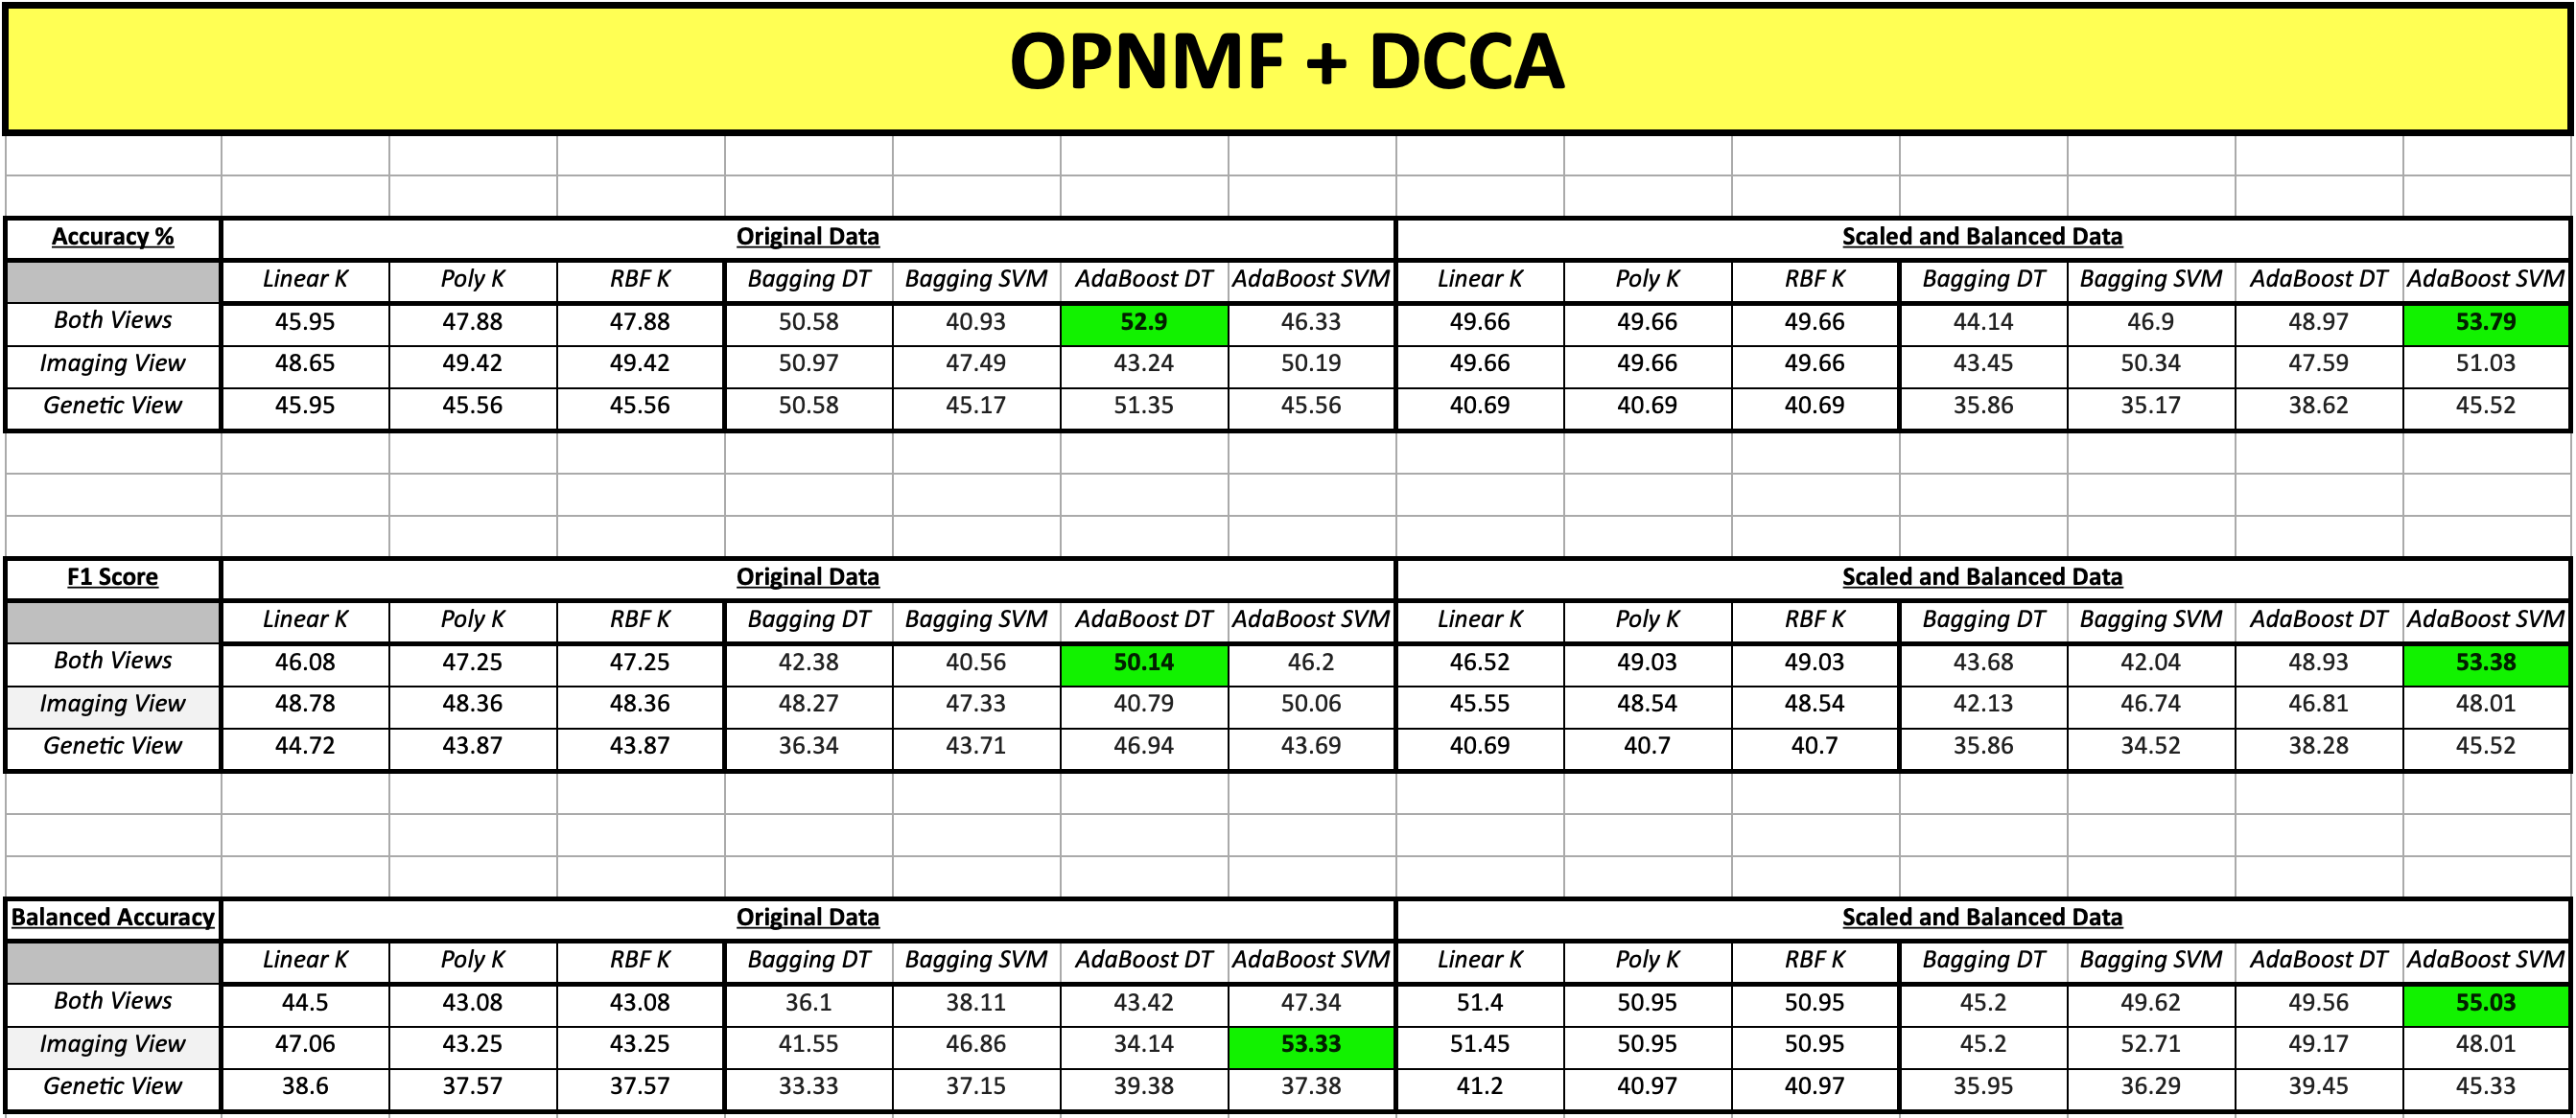
\includegraphics[width=\textwidth]{figures/Results/Analytical_Table_OPNMF_DCCA.png}
    \caption[\en{Analytical table of results for OPNMF - DCCA transformed data classification}]{\en{For each model and classifier, the metric scores for OPNMF - DCCA transformed data classification are presented. Highlighted green are the best performing models, for each metric.}}
    \label{fig: Summary Table for classification scores for OPNMF - DCCA transformed data}
\end{figure}
}